\documentclass{article}

\usepackage[utf8]{inputenc}
\usepackage[T1]{fontenc}
\usepackage{fourier}
%\usepackage[latin1]{inputenc}
\usepackage[spanish]{babel}

\usepackage[thinlines]{easytable}
\usepackage{diagbox}
\usepackage{multirow}


\usepackage[protrusion=true,expansion=true]{microtype}	
\usepackage{amsmath,amsfonts,amsthm} % Math packages
\usepackage{amssymb}
\usepackage[pdftex]{graphicx}	
\usepackage{url}
\usepackage{tikz}
\usepackage{setspace}
\usepackage{import}
\usepackage{float}
\usepackage{graphicx}
\pagenumbering{arabic}
%margenes 
\usepackage{geometry}
 \geometry{
 a4paper,
 left=19mm,
 right=19mm,
 top=19mm,
 bottom=42mm,
 }

% %%% Custom sectioning
\usepackage{sectsty}
%\allsectionsfont{\normalfont \scshape}


%%% Custom headers/footers (fancyhdr package)
\usepackage{fancyhdr}
\pagestyle{fancyplain}
\fancyhead{}											% No page header
\fancyfoot[L]{}											% Empty 
\fancyfoot[C]{}											% Empty
\fancyfoot[R]{\thepage}									% Pagenumbering
\renewcommand{\headrulewidth}{0pt}			% Remove header underlines
\renewcommand{\footrulewidth}{0pt}				% Remove footer underlines
\setlength{\headheight}{13.6pt}


%%% Equation and float numbering
\numberwithin{equation}{section}		% Equationnumbering: section.eq#
\numberwithin{figure}{section}			% Figurenumbering: section.fig#
\numberwithin{table}{section}				% Tablenumbering: section.tab#


%%% Maketitle metadata
\newcommand{\horrule}[1]{\rule{\linewidth}{#1}} 	% Horizontal rule

\begin{document}
\onehalfspacing

\begin{titlepage}
    
\newcommand{\HRule}{\rule{\linewidth}{0.5mm}} % Defines a new command for the horizontal lines, change thickness here
    
\center % Center everything on the page
     
%----------------------------------------------------------------------------------------
%	HEADING SECTIONS
%----------------------------------------------------------------------------------------
    
\textsc{\LARGE Instituto Tecnológico de Buenos Aires}\\[2cm] % Name of your university/college
\textsc{\Large 22.42 Laboratorio de Electrónica}\\[1.5cm] % Major heading such as course name
\textsc{\large Trabajo Práctico N° 2}\\[0.5cm] % Minor heading such as course title
    
%----------------------------------------------------------------------------------------
%	TITLE SECTION
%----------------------------------------------------------------------------------------
    
\HRule \\[0.5cm]
{ \huge \bfseries Osciloscopios/ Analizador de Impedancias/ \\Circuitos RLC}\\[0.4cm] % Title of your document
\HRule \\[2cm]
     
%----------------------------------------------------------------------------------------
%	AUTHOR SECTION
%----------------------------------------------------------------------------------------
    
\begin{minipage}{0.4\textwidth}
\begin{flushleft} \large
\emph{Grupo 5:}\\		%names
[.3cm]
Nicolás \textsc{De León}\\
Leg. 57232\\ 
[.3cm]
Tomás \textsc{Vigón}\\
Leg. 57327\\ 
[.3cm]
Benjamín \textsc{Lin}\\
Leg. 57242 \\ 
[.3cm]
Lucero Guadalupe \textsc{Fernandez}\\
Leg. 57485\\ 
[.3cm]
\end{flushleft}
\end{minipage}
~
\begin{minipage}{0.4\textwidth}
\begin{flushright} \large
\emph{Profesor:} \\
[.3cm]
Pablo  \textsc{Cossutta}\\ % Supervisor's Name
Alejandra \textsc{Weill} \\% Supervisor's Name
Matías  \textsc{Salvati} % Supervisor's Name
\end{flushright}
\end{minipage}\\[2cm]
    
%----------------------------------------------------------------------------------------
%	DATE SECTION
%----------------------------------------------------------------------------------------
    
\vfill
{\large Entregado: 25 de Septiembre de 2018}\\[2cm]
    
\vfill 
    
\end{titlepage}

\section{Análisis de circuito RC}

Se armó el circuito de la figura inferior con los valores nominales de $R=3.9k\Omega$ y $C=1.8nF$.
\begin{figure}[h!]
\centering
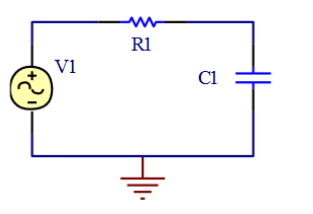
\includegraphics[scale=0.5]{rcCircuito.png}
\caption{Circuito RC armado.}
\label{fig:RC}
\end{figure}

\subsection{Cálculo de Frecuencia de Corte}

La frecuencia de corte es aquella en la que la salida $V_{out}$ atenúa la entrada $V_{in}$ en $-3dB$ y la primera desfasa a la segunda en $45^o$; de esta manera
se buscó experimentalmente su respectiva frecuencia de corte que resultó ser $f_{cmedido}=21.8kHz$. Se tuvo en cuenta la resistencia interna
del generador ($50\Omega$), y se la sumó a la $R_{teorica}$ .

A continuación, sabiendo que $C_{cal}\text{=}\frac{1}{2\pi fR}$ se completó la siguiente tabla:

\begin{table}[!htb]
\centering
\begin{tabular}{|c|c|c|c|c|c|}
\hline 
$|V_{in}|[V]$ & $|V_{out}|[V]$ & $R[k\Omega]$ & $C_{calculado}[nF]$ & $C_{medido}[nF]$ & $Error\%$\\
\hline 
\hline 
4.97 & 3.46 & 3.95 & 1.775 & 1.848 & 3.95\\
\hline 
4.97 & 3.46 & 3.93 & 1.784 & 1.848 & 3.46\\
\hline 
\end{tabular}
\caption{Tensiones y valores de componentes del circuito.}
\end{table}

\subsection{Medición de ángulo de fase entre I y $V_C$}

Para el cálculo de la corriente se utilizó $I=\frac{V_{R}}{R}$, asumiendo que la tensión y la corriente de la resistencia estaban en fase. 
Luego con el uso de la opción math del osciloscopio, se restó la caída en el capacitor a la tensión de entrada y se midieron las fases y amplitudes de las mismas, siendo la resultante de la resta $V_R$. Una vez que se obtuvo, se la dividió por el valor de la resistencia, obteniendo así, el valor vectorial de la corriente.
De esta manera se obtuvo que $|V_{R}|=3.51V$ y $|V_{c}|=3.48V$.

\begin{figure}[H]
\centering

\includegraphics[scale=0.5]{1-2.png}
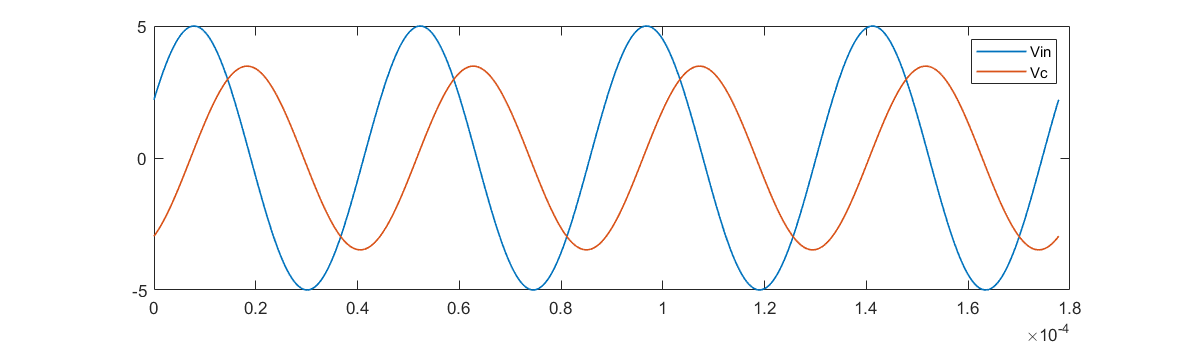
\includegraphics[scale=0.5]{1-2b.png}
\caption{Diagrama fasorial y representación de las señales VR y VC.}
\label{diagfasorial}
\end{figure}


De la figura \ref{diagfasorial} observamos que la corriente se adelanta a la tensión del capacitor $90^{o}$. Ademas, la suma fasorial de $V_R$ y $V_C$ es de 4.97V en vez de los 5V, esto puede ser por la resistencia del generador que aún siendo pequeña genera una caída de tensión en el circuito.

\subsection{Cálculo analítico de la función transferencia}

Teniendo en cuenta la fiugra \ref{RC}; con $V_{out}$ la tensión del capacitor y $V_{in}$ como la tensión de entrada que fue una senoidal de $5~V_{pp}$, se halló analíticamente la función transferencia planteando un divisor resistivo, que resultó ser:

\begin{center}
\begin{equation}
\label{transf}
H(s)=\frac{1}{sRC+1}
\end{equation}
\end{center}

siendo $s=j\omega$ y $R=R_{medida} + R_{generador}$.

La frecuencia de corte resulta ser el polo de la función, es decir, cuando 
$\omega_c=\frac{1}{RC}$. Entonces, teniendo en cuenta que $\omega=2\pi f$, se deduce que la frecuencia de corte es $f_{ccalculado}=22.75kHz$. 
Se puede ver que la función obtenida es un pasabajos con un polo simple en $\frac{1}{2\pi RC}$.
Se diagramó el Bode de magnitud y fase, que se muestra a continuación.

\begin{figure}[H]
\centering
\begin{minipage}{.5\textwidth}
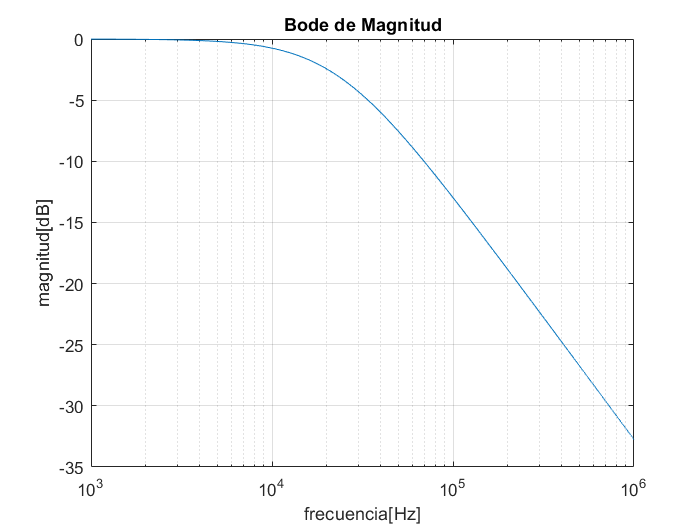
\includegraphics[scale=0.45]{1-3a.png}
\end{minipage}%
\begin{minipage}{.5\textwidth}
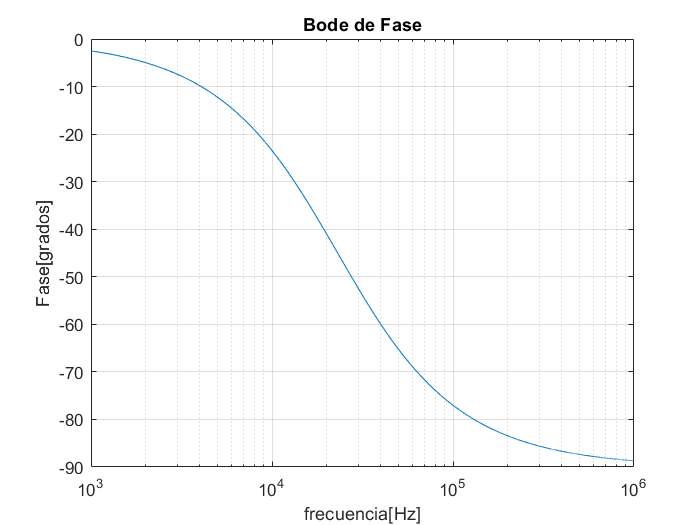
\includegraphics[scale=0.45]{1-3b.png}
\end{minipage}
\caption{Bode de magnitud y fase para los valores medidos de R y C.}
\label{diagbodemedido}
\end{figure}


En la figura \ref{diagbodemedido} puede verse que la frecuencia en la que la ganancia del circuito es $-3dB$ y el desfase es de $45^o$ es la frecuencia de corte, que ronda los 22.7kHz.

\subsection{Función transferencia a distintas frecuencias}

Se midieron valores de tensión y fase a distintas frecuencias entre 10Hz y 1MHz, completando la siguiente tabla. Donde el ángulo $\varphi_1$ fue medido en el modo $\Delta t$ del osciloscopio; y el ángulo $\varphi_2$, en el modo XY del osciloscopio.
//VALOR DE TENSION? 
La diferencia entre ambos $\varphi$ se debe a errores de apreciación al medir y de cálculo al realizar $\arcsin(\frac{\Delta X}{\Delta Y})$, siendo $\Delta X$ el ancho mínimo entre 2 extremos de la elipse y $\Delta Y$ el ancho máximo entre dos de ellos. 

\label{tablabode}

\subsection{Bode teórico y empírico}
Se graficó lo obtenido de la tabla \ref{tablabode} y se lo superpuso con el diagrama de Bode teórico de la función transferencia (ecuación \ref{transf}).

\begin{figure}[H]
\centering
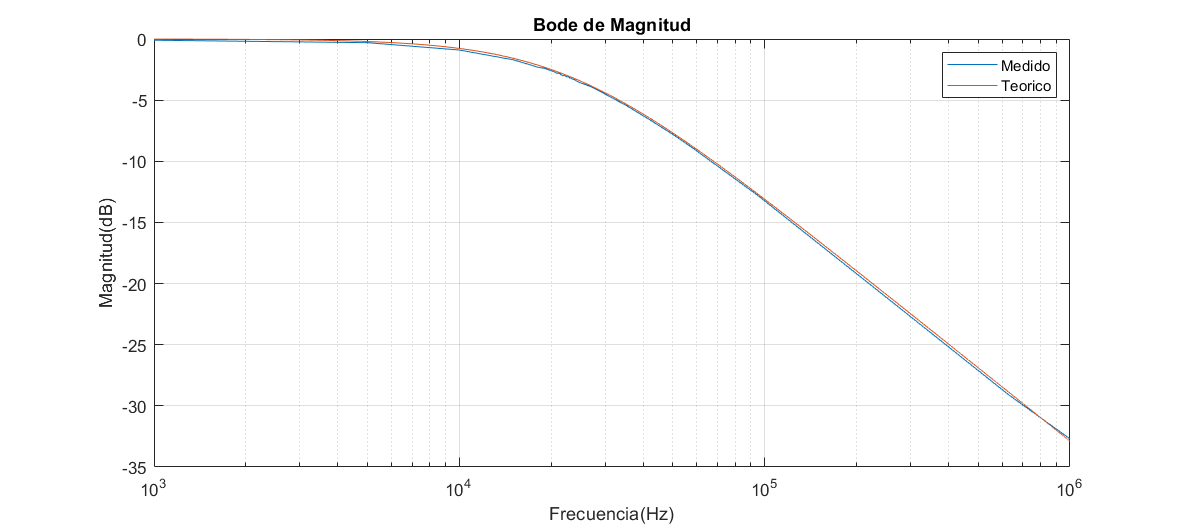
\includegraphics[scale=0.4]{1-4a.png}
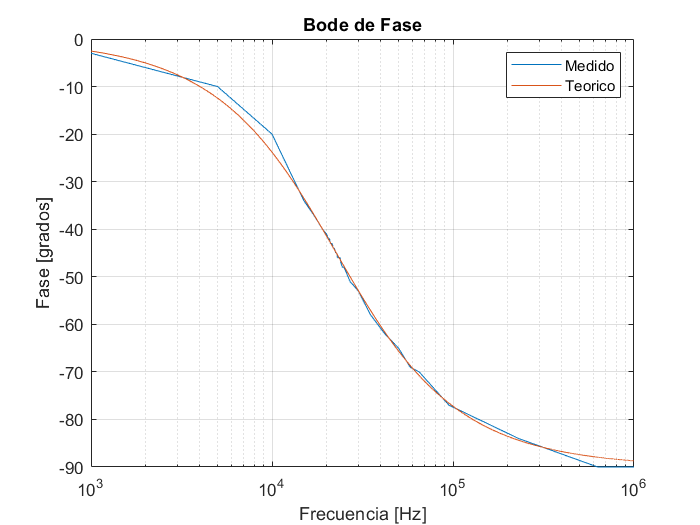
\includegraphics[scale=0.5]{1-4b.png}
\caption{Bode de magnitud y fase medido y teórico.}
\label{diagbode}
\end{figure}

Se puede observar que para el diagrama de amplitud las mediciones a distintas frecuencias se corresponden a lo calculado teóricamente. En el diagrama de fase, las variaciones se deben a errores de medición y en el rango de frecuencias altas, donde la señal es atenuada. se encuentra un mayor error ya que el ruido se hace comparable con las mediciones.

\subsection{Respuesta al escalón}

\begin{figure}[H]
\centering
\subfloat[Frecuencia 1kHz.]{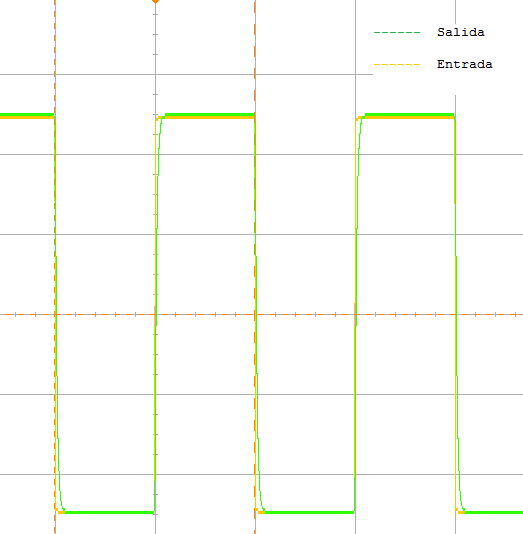
\includegraphics[scale=0.35]{1ka.png} }%
\qquad
\subfloat[Frecuencia 15kHz.]{{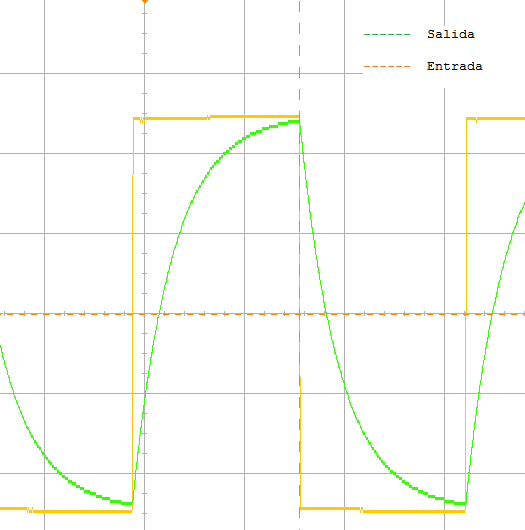
\includegraphics[scale=0.35]{15ka.png} }}%
\qquad
\subfloat[Frecuencia 200kHz.]{{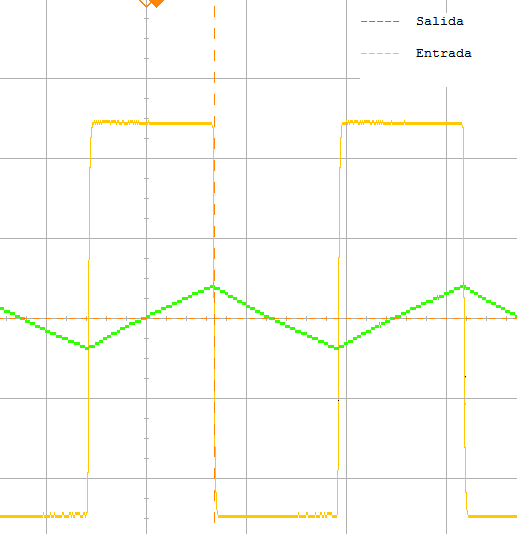
\includegraphics[scale=0.35]{200ka.png} }}%
\caption{Respuesta al escalón.}
\label{diagbodemedido}
\end{figure}

\textbf{1.8}
//1.7
//imagenes 1.8

\textbf{1.9 Conclusiones}

\section{parte2}

\section{Respuesta en frecuencia con barrido automático}

\subsection{Modo normal del osciloscopio}

El barrido automático se realizó con el generador en donde se barrió
de 100Hz a 2MHz en un lapso de 100 mili segundos con una senoidal
de 20 $V_{pp}$. El output del generador se utilizó para excitar al
circuito RC y se conectó el sync al osciloscopio para poder triggerear
la señal, además se aprovechó el marker del sweep del generador para
que la cuadrada entregada por el sync tenga un ancho de 22,6KHz para
que coincida con la frecuencia de corte calculada de nuestro circuito.
Cabe mencionar que el barrido automático estaba configurado en escala
logaritmica. Se obtuvó la siguiente imagen:

\begin{figure}[H]
\begin{center}
%\includegraphics[bb = 0 0 200 100, draft, type=eps]{./Respuesta en frecuencia barrido automatico modo normal.png}
\par\end{center}
\caption{Respuesta en frecuencia con barrido automatico en modo normal}
\end{figure}

La figura evidencia claramente el efecto del filtro pasa bajos sobre
el circuito, mientras que la señal amarilla que es la entrada se
mantiene constante en amplitud a lo largo de todo el barrido, la salida
que es la senial verde tiene ganancia unitaria en las bajas frecuencias
y luego se atenua a medida que esta aumenta. La senial cuadrada violeta
marca la frecuencia de corte del circuito donde se espera una caida
de 3dB. En veces equivale aproximadamente a una atenuacion de $\sqrt{2},$es
decir, $V_{0}=\sqrt{2}V_{i}$ y en nuestro caso como $V_{i}$ tiene
una amplitud de 10 V, $V_{0}$ deberia tener una amplitud aproximada
de 7,1 V, esto se puede observar claramente en el gráfico.

\subsection{Modo XY del osciloscopio}

Se intento de siumular el barrido en el modo XY bajo ciertas características.
Se colocó un generador realizando un sweep barriendo nuevamente frecuencias
de $100Hz$ a $2MHz$ esta vez linieal cada $10ms$ con una senoidal
$20Vpp$ y bajo estas condiciones se lo conectó a la entrada del circuito.
Luego se sincronizó el trigger del generador de sweep con el flanco
descendente de la señal del generador 2, en el cual se colocó una
rampa de $10Vp$ a una periodo de $11ms$ y se la conectó en la entrada
X del osciloscopio. Se conectó la salida del circuito a la entrada
Y del osciloscopio. Por consecuente, tomando en cuenta las consideraciones
establecidas, se esperaba ver como en el modo XY el eje Y iba a presentar
las senoidales en modo sweep desde la frecuencia inicial a la final
y en la componente X un desplazamiento de 0 a 10V estableciendo la
relación $0V$ a $t=\text{0}$ y en $10V$ $t=11ms$ dejando entrar
un poco mas de un barrido en pantalla.
\begin{figure}[H]
\centering{}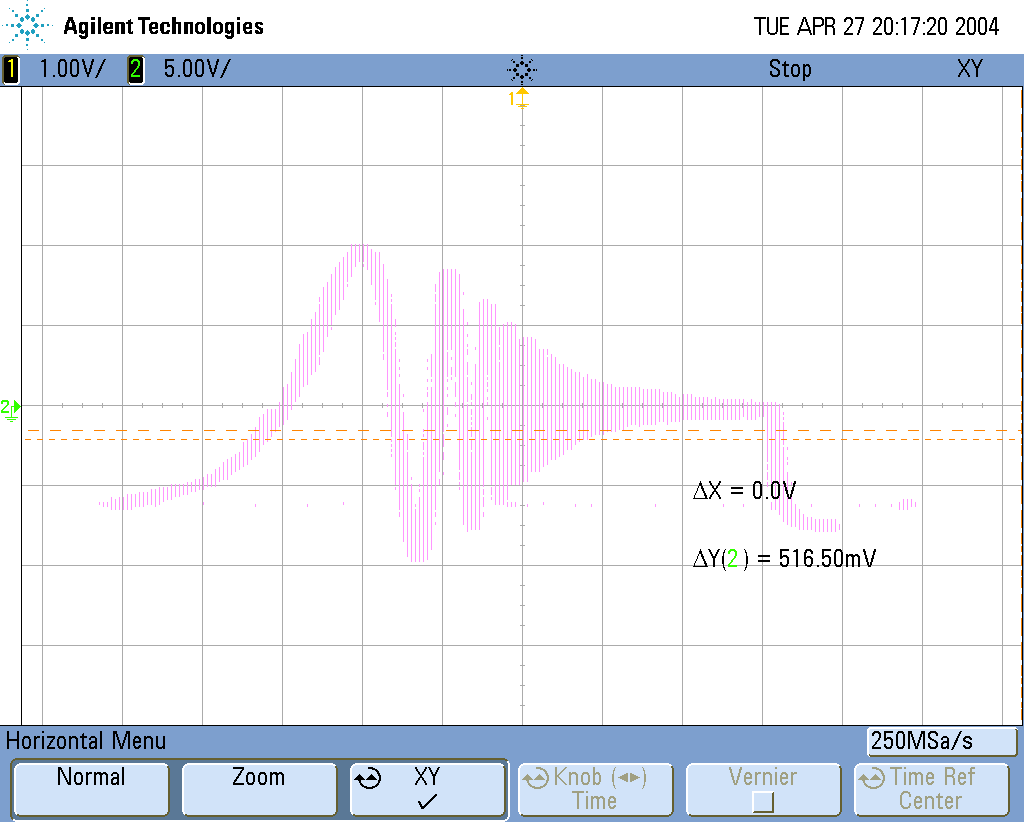
\includegraphics{./scope_24.png}\caption{Respuesta en frecuencia con barrido automático en modo XY}
\end{figure}

Se puede observar como las configuraciones previas permitieron el
análisis en frecuencia del circuito, dando una imagen relacionada
directamente con la obtenida en el modo normal del osciloscopio bajo
el mismo sweep. Es importante notar como se configuró la escala en
X y en Y para poder formar correctamente la imagen en pantalla del
barrido en frecuencia.

\section{Respuesta en frecuencia del osciloscopio}

Para medir la respuesta en frecuencia del osciloscopio se utilizaron
dos puntas de osciloscopio y un generador, por un lado se conectaron
ambas puntas con el generador de seniales entre sí y por el otro las
masas de estos tres elementos también entre sí. El bode del circuito
se realizó con los filtros AC y el BW del osciloscopio activados y
se lo excitó con una senoidal de 10 $V_{pp}$. Los resultados obtenidos
de las mediciones se graficaron en la siguiente figura:
\begin{figure}[H]
\caption{Respuesta en frecuencia del osciloscopio}
\end{figure}

Se puede observar que la forma de la respuesta en frecuencia es la
de un filtro pasa banda ya que atenua las frecuencias menores a 12Hz
y las frecuencias mayores a 5MHz. Esto se debe a que el filtro AC
del osciloscopio filtra las seniales continuas con un capacitor formando
un pasa altos que posee una frecuencia de corte muy pequenia; y el
filtro BW dismunuye el ancho de banda atenuando las altas frecuancias
mediante un filtro pasa bajo, la combinación de ambos actuan como
el pasa banda representado en la figura 1.
\end{document}
